\subsection{Scoring}

\paragraph{}
Also within the input file are some scoring options. In FLUKA, the \textit{measurables} are \textit{scored} or synonymously, \textit{estimated}. Nevertheless, the scoring section of the input file contains a few cards activating the builtin scoring features of FLUKA, and another single card that requests the custom scoring from within the ``mgdraw.f'' file.

\begin{figure}[h]
    \begin{center}
    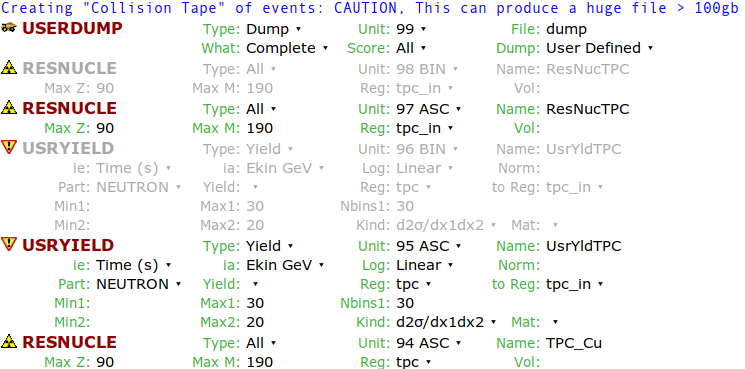
\includegraphics[scale=0.5]{figures/scoring.png}
    \caption{The set of scoring cards in the nEXO input file}
    \label{fig:scoring}
    \end{center}
\end{figure}

\paragraph{}
In figure \ref{fig:scoring} there is the entirety of the scoring section in the input card. The \textcolor{Maroon}{USERDUMP} card specifies that the ``mgdraw.f'' routine gets called to enable the customized scoring therein. However, one has to be careful as the default ``mgdraw.f'' file can save \textbf{much} more data than is necessary resulting in files exceeding tens of gigabytes in size— hence the \textcolor{Blue}{comment} above the card.

\paragraph{}
The \textcolor{Maroon}{RESNUCLE} cards tell FLUKA to print out ascii (human-readable) files which contain the counts of residual nuclei in a given region. Seen here we have cards for the TPC liquid xenon and also the copper TPC shell. 

\paragraph{}
Data from the other scoring cards are not currently used but they can be used to score differential fluence (with respect to energy, time, etc...). In essence all one needs for the nEXO scoring are the residual nuclei scoring cards for activation, and the USERDUMP which sends the data to the custom routine that takes care of the rest of the neutron data.